% A simple template for LaTeX documents
% 
% To produce pdf run:
%   $ pdflatex paper.tex 
%

\documentclass[12pt]{article}

% Begin paragraphs with new line
\usepackage{parskip}  

% Change margin size
\usepackage[margin=1in]{geometry}   

% Graphics Example:  (PDF's make for good plots)
\usepackage{graphicx}               
% \centerline{\includegraphics{figure.pdf}}

% Allows hyperlinks
\usepackage{hyperref}

% Blocks of code
\usepackage{listings}
\lstset{basicstyle=\ttfamily, title=\lstname}
% Insert code like this. replace `plot.R` with file name.
% \lstinputlisting{plot.R}

% Supports proof environment
\usepackage{amsthm}

% Allows writing \implies and align*
\usepackage{amsmath}

% Allows mathbb{R}
\usepackage{amsfonts}


%%%%%%%%%%%%%%%%%%%%%%%%%%%%%%%%%%%%%%%%%%%%%%%%%%%%%%%%%%%%
\begin{document}

\title{US Korea Exchange Rates \\ STA206 Final Project}
\date{December 15, 2014}
\author{Clark Fitzgerald clarkfitzg@gmail.com \\ 
        Amy Kim atykim@ucdavis.edu}

\maketitle

\begin{abstract}
    We analyze the exchange rate between the United States and South Korea
    using monthly country level economic data.
\end{abstract}

\section{Introduction}

\section{Methods and Results}

Figure~\ref{fig:correlation} shows a histogram of all the pairwise sample
correlations.

Figure~\ref{fig:na_plot_KOR} shows the variables which were interpolated.

\section{Conclusions and Discussion}


\newpage
\section{Appendix}

\listoffigures

\begin{figure}
  \centering
    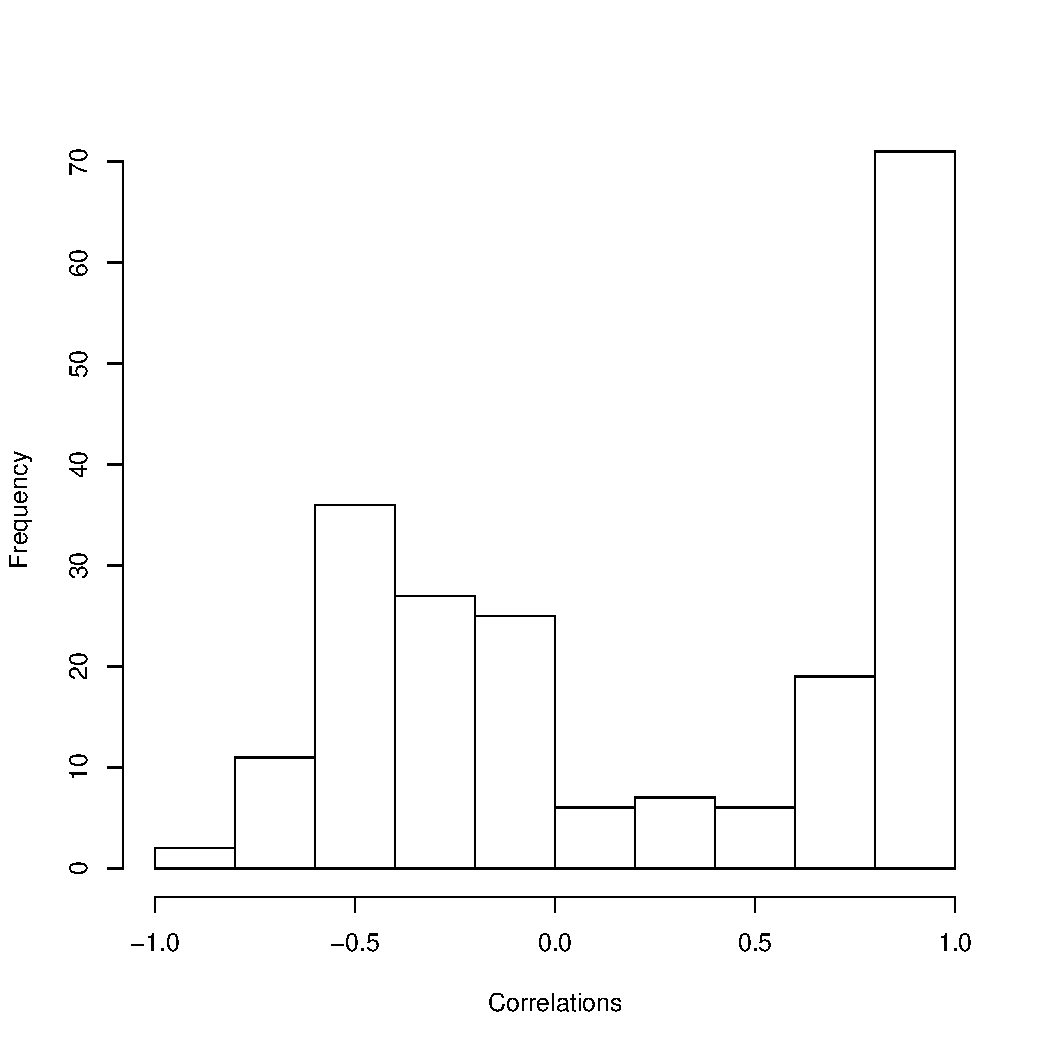
\includegraphics{correlation.pdf}
  \caption{Histogram of all pairwise sample correlations.}
  \label{fig:correlation}
\end{figure}

\begin{figure}
  \centering
    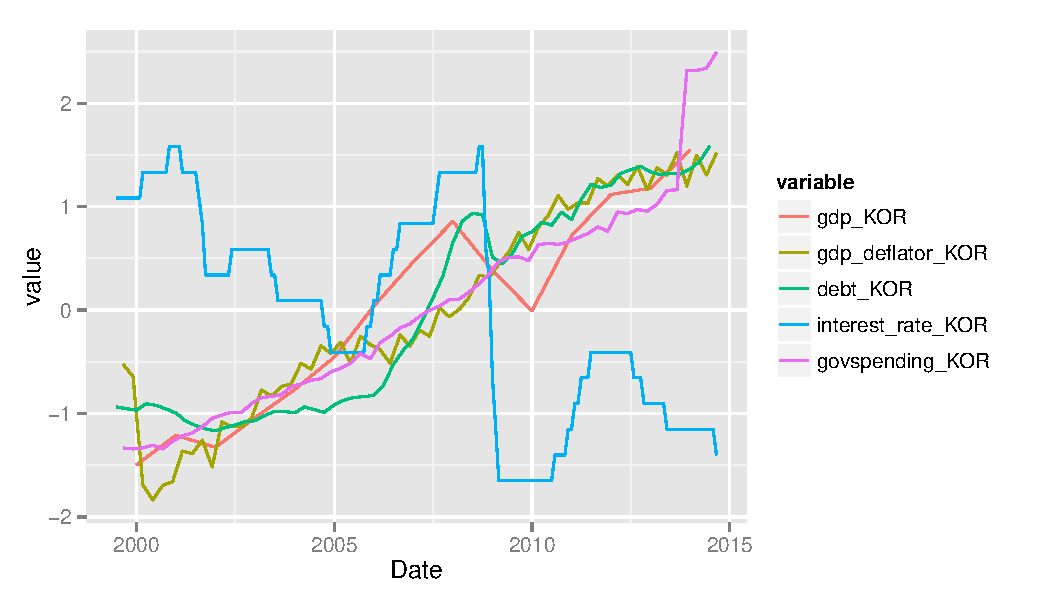
\includegraphics{na_plot_KOR.pdf}
  \caption{Scaled variables with NA values.}
  \label{fig:na_plot_KOR}
\end{figure}

\end{document}
